\chapter{Experiment and Results}
\label{expres}

After a considerable amount of research in clustering and metric learning, we chose triplet loss as our method of approaching the problem. Triplet loss is a  well-established, simple and effective when it comes to learning a latent space. Other methods such as the one proposed by \citet{lifted_structure_embedding} were overly complicated, especially given the size of our dataset. Triplet loss was relatively easy to implement given how we organized the transformed data and so, a network trained on triplet loss was the natural choice for this experiment. 

\section{Initial Experiments}

Initially, we did not know whether this method would work on the STFT transformed signals as described in \cref{data} and we needed a simple way to test out the concept. Hence, to learn the latent space, we needed to start with a relatively simple network. 

Although the network's architecture was not a priority since this was only a test run of the concept, CNNs were considered from the very beginning since they perform very well in image and video processing tasks as mentioned in \cref{cnns}. Spectrograms inherently look like images as we saw in \cref{fig:stft}. Since we are using spectrograms of the EEG signals as the input, it made sense to use CNNs. Secondly, we assumed that the labels for each second of each channel of original signal were properly time-aligned in the time domain. In case that this assumption is invalid, CNNs still can perform better than other types of networks. CNNs tend to learn the patterns in the spectrogram even if they were not time-aligned since they learn shift-invariant features. Hence, an important feature that starts in the first interval of the spectrogram may still be recognized even if it starts sixty intervals later.

\begin{table}[!ht]
	\centering
	\small
	\caption{Network architecture for CNN}
	\begin{tabular}{rllc}
		\toprule
		Layer    & Input                     & Output                    & Kernel       \\ \midrule
		conv1  & $ 71 \times 125 \times 1 $  & $ 71 \times 125 \times 32 $ & $ 4 \times 4 $ \\
		pool1  & $ 71 \times 125 \times 32 $ & $ 35 \times 62 \times 32 $  & $ 3 \times 3 $ \\
		conv2  & $ 35 \times 62 \times 32  $ & $ 35 \times 62 \times 64 $  & $ 5 \times 5 $ \\
		pool2  & $ 35 \times 62 \times 64 $  & $17 \times 30 \times 64$    & $ 2 \times 2 $ \\
		fc1    & $17 \times 30 \times 64$    & $ 256          $            & N/A            \\
		fc2    & $ 256 $                     & $ 128 $                    & N/A            \\
		output & $ 128 $                    & $ 64   $                    & N/A            \\ \bottomrule
	\end{tabular}
	\label{tab:network}
\end{table}

Eventually, we built our initial model described in \cref{tab:network} in TensorFlow as described by \citet{tensorflow}. The  code in \cref{initial_model_code} was used to build the network described. We trained the initial model on a Lenovo Y700 laptop running Ubuntu $16.06$ LTS with an Intel Core i7-6700HQ CPU running at $2.60$ GHz, $8$ GB of RAM and no discrete graphics card for Tensorflow's CUDA acceleration capabilities. 

In our first attempt, the loss function converged to values very close to zero within the first few iterations. After stepping through the code, we discovered that the input data values were all in the $10^{-5}$ order of magnitude. As a result, the network was discovering a trivial solution that would satisfy the loss function and at the same time not solve the problem at hand. In order to avoid this, we amplified the input data by multiplying all inputs to the network by $10^4$. The network started to train normally and we noticed that the network's loss started to decrease. Semi-hard or hard triplets were chosen at run-time to train the network. Any ``soft'' triplets were skipped until semi-hard or hard triplets were found since they do not contribute to the learning of the space. 

\subsection{Hyperparameter Selection}

Initially, we had selected random hyperparameters for the network. Once we realized that the network started to train as we intended it to, we needed to select the hyperparameters the learning rate, $\eta$, the margin parameter, $\alpha$, the regularization strength, $\lambda$ and the output dimension, $d$. More attention was given to $\eta$ since we wanted the network to converge fast but not oscillate before reaching convergence. Despite using the Adam optimizer, the oscillation described in \cref{paramsmodeling} can still occur due to small, deep valleys in the hypersurface created by the loss function. In most experiments that we've seen, $\lambda$ is typically a magnitude below the learning rate. We continued that convention and selected $\eta = 10^{-3}$ and $\lambda=10^{-4}$. Regularization was not necessarily important at this point so not much attention was given to $\lambda$.  The rest of the parameters were chosen to be ``nice'' numbers and were $\alpha = 1.0$, and $d=128$.  

We attempted running the network for a hundred thousand iterations. However, we noticed that after fifty thousand iterations, the triplet mining process was slowed down because the script found it difficult to find semi-hard or hard triplets. At one point, we observed that nearly two hundred thousand triplets were skipped due to their soft nature. Due to this phenomenon, we hypothesized that the network had started to converge at around sixty thousand iterations and decided that it was no longer needed to train. After that point, this particular network architecture was trained for sixty thousand iterations and the data pool was changed every ten thousand iterations to help the script find more semi-hard or hard triplets. This alleviated the stalling nature of triplet mining. 

% We tried to further fix this problem by changing the margin parameter to $\alpha=0.5$ and decreased the output dimension to $d=64$ to see the differences in the results. We found that both set of hyperparameters gave similar results and therefore we utilized the latter set since it was more compressed than the former.

\subsection{Measuring Performance}

Although the loss was decreasing as expected, we needed a way of validating whether the space that we anticipated was actually forming. One way to do this was to follow the advice given by \citet{facenet} and use a k-NN classifier to quantify the quality of the embedding space produced. Assuming that the data provided was classified correctly, we run some training data through the network to find the embeddings of those samples. We then populate the k-NN space with those embeddings. New embeddings produced from the validation set are introduced to the k-NN algorithm and classified. Theoretically, if the embedding space develops distinct clusters based on the classes, it would classify the validation signals with a relatively high overall accuracy since the validation set's embeddings would be near the cluster.  

We used SciKit Learn's implementation of the k-NN classifier to apply the test described. The default value of the number of neighbors, $k=5$, was used to classify the validation embeddings produced. This test resulted in an $80\%$ accuracy. At this point, we were not using stratified sampling to adjust for the data imbalance. Hence, we assumed that most of the data that was classified incorrectly were originating from classes with low numbers of samples points. It was clear that the experiment was a success and our initial hypothesis that triplet loss can be used learn a latent space for EEGs was valid since the resulting accuracy was relatively high considering that we only used a very simple, two-layer CNN.

\subsection{Error in Dataset Organization}

Unfortunately, the success that we experienced with the initial network was not long-lasting. When we explored the various sources of errors in the experiment, it was obvious that the amount of time used to train the network and the overall accuracy of the network was qualitatively low and high, respectively. Therefore, we tried to inspect the code used so far for any possible errors that we may have introduced. We discovered that the data used to train the network was organized in a way such that the different classes of data was easily split, but the patients, i.e. the different sessions, were not. Therefore, when training, we were implicitly training and validating on a portion of the training set which was already seen. 

Our goal was to make this system general so that the system can detect the presence of any of the six signals in any patient, not only for the patients provided in the dataset. Hence, it was necessary for us to reorganize the data so that it was split by session \textit{and} class. We split the dataset again so that sessions from \verb+session1+ until \verb+session300+ were used as training data and the rest of the sessions were used as testing data while retaining all information about the signal including session, type of signal and time of the signal in the session. This ensured that the training set and the validation set were truly mutually exclusive. Furthermore, the new method of organization helped in conducting analysis of files with seizure-like signals and files with noise-like signals which will be discussed in \cref{analysis}.

\section{DCNN with Triplet Loss}

As discussed in \cref{bias_variance_tradeoff}, it is generally easier to cut down a model by using regularization than it is to increase the complexity of a model. Since the concept of using triplet loss to train a CNN for clustering EEG signals was validated, it made sense to proceed to the next step and experimentally increase the complexity of the network. The next logical step from two-layer CNN was to make a DCNN that used multiple layers of convolution to learn more complex shift-invariant features.

We continued the same convolutional layer followed by maxpool layer pattern with a fully connected layer at the end, as seen in the initial network shown in \cref{tab:network}. Our new network, specified in \cref{tab:dcnn}, consisted of five convolutional layers each followed by a maxpool layer. We built the network using Tensorflow again and trained the model on a server with Intel Xeon ES-2620 24-core CPU with each core at $2.10$ GHz, $128$ GB of RAM and five Nvidia GeForce Titan X GPUs with $12$ GiB of video memory for Tensorflow's GPU acceleration.

\begin{table}[!ht]
	\centering
	\small
	\caption{Network architecture for simple CNN}
	\begin{tabular}{rllc}
		\toprule
		Layer    & Input                     & Output                    & Kernel       \\ \midrule
		conv1    & $71 \times 125 \times 1$  & $71 \times 125 \times 32$ & $5 \times 5$ \\
		maxpool1 & $71 \times 125 \times 32$ & $34 \times 61 \times 32$  & $5 \times 5$ \\
		conv2    & $34 \times 61 \times 32$  & $34 \times 61 \times 64$  & $3 \times 3$ \\
		maxpool2 & $34 \times 61 \times 64$  & $16 \times 30 \times 64$  & $3 \times 3$ \\
		conv3    & $16 \times 30 \times 64$  & $16 \times 30 \times 128$ & $2 \times 2$ \\
		maxpool3 & $16 \times 30 \times 128$ & $8 \times 15 \times 128$  & $2 \times 2$ \\
		conv4    & $8 \times 15 \times 128$  & $8 \times 15 \times 256$  & $1 \times 1$ \\
		maxpool4 & $8 \times 15 \times 256$  & $4 \times 7 \times 256$   & $2 \times 2$ \\
		conv5    & $4 \times 7 \times 256$   & $4 \times 7 \times 1024$  & $4 \times 4$ \\
		maxpool5 & $4 \times 7 \times 1024$  & $1 \times 2 \times 1024$  & $4 \times 4$ \\
		flatten  & $1 \times 2 \times 1024$  & 2048                      & N/A          \\
		fc1      & 2048                      & 1024                      & N/A          \\
		fc2      & 1024                      & 512                       & N/A          \\
		fc3      & 512                       & 256                       & N/A          \\
		output   & 256                       & 64                        & N/A          \\ \bottomrule
	\end{tabular}
	\label{tab:dcnn}
\end{table}


\subsection{Hyperparameter Selection}
The architecture of the network itself can be varied and may be considered a hyperparameter by itself. We can vary the number of layers, the number of neurons in each layer, the convolutional kernel size, the activation functions, parameter initialization methods and so on. However, this is something that is developed with experience in the field. There are ways to make some of those hyperparameters learnable. For example, the work done by \citet{inception} allows a single convolutional layer to have variable kernel sizes. When using backpropagation, the network can learn which kernels are used and how much they are used in determining the final output. \citet{prelu} work on the parametrization of the ReLU activation function in order to help learn what type of activation function is optimal for a given task. However, such ways of improving the architecture are outside of the scope of this thesis and introduces more issues that increase the overall complexity of the network. 

Following the results of the initial experiment, we started to train the new network with the same hyperparameters as the network shown in \cref{tab:network} and decided to pivot on the hyperparameters as necessary in order to find the best model that both generalizes well to the validation set and forms a relatively compressed latent space. We did a manual grid search on a particular range for each of the hyperparameters, $\eta$, $\alpha$, $\lambda$ and $d$. We cross-validated the networks' ability to infer what new signals might be by using the validation set that we had set aside. After training the network and cross-validating, it was found that $\eta=10^{-4}$ , $\alpha=0.5$, $\lambda = 10^{-3}$ and $d=64$ led to the best results. 

\subsection{Measuring Performance}

We still used k-NN classification accuracy as a measure of the quality of the latent space produced. However, in order to make sure that the classification was being done correctly, we elected to change the number of neighbors that the k-NN algorithm used to a higher value. Increasing $k$ effectively smoothens the decision boundary since the algorithm uses more neighbors to make its decisions. After experimentally increasing the number of neighbors the algorithm considered to make the classification decision in the latent space, we chose $k=31$ as it had the highest level of accuracy and completed the task quickly with the amount of available memory.  With those hyperparameters, we achieved a validation accuracy of $60.4\%$. The confusion matrix for that iteration of cross-validation is shown in \cref{fig:dcnnlarge}. 

\begin{figure}[!ht]
	\centering
	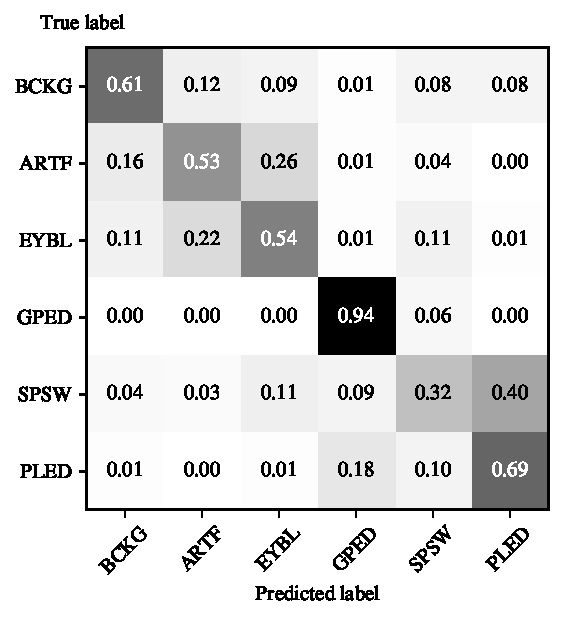
\includegraphics[width=0.55\linewidth]{pictures/conf_mat_exp.pdf}
	\caption[Confusion matrix for the DCNN clustering network]{Confusion matrix for the DCNN clustering network with $\alpha = 0.5$, $\eta = 10^{-5}$ after $105$k iterations, and an accuracy of $60.4\%$ with 31-NN classification}\label{fig:dcnnlarge}
\end{figure}

The classification accuracy provides a numerical value which could be used as a measure of the quality of the embedding that our system produces. However, this does not necessarily provide us information on whether clusters are forming, which is what we were hoping would happen from the beginning. In order to test how well the network was doing in clustering signals based on similarity, we decided to apply t-distributed stochastic neighbor embedding  (t-SNE\nomenclature{t-SNE}{t-Distributed Stochastic Neighbor Embedding}) which is an algorithm that reduces the dimensionality of high dimensional data. Although this algorithm reduces the dimensionality, the overall structure of the latent space remains the same as the structure of the $d$-dimensional latent space. If clusters exist in the t-SNE plot, it would mean that the same clusters are highly likely to exist in the $d$-dimensional latent space. Hence, we used t-SNE to visualize the $64$ dimension latent space in $2$D. The t-SNE reduced two dimensional embedding after $5$k iterations is shown in \cref{fig:tsne_start} and the same after $105$k iterations is shown in \cref{fig:tsne}. 

\begin{figure}[!ht]
	\centering
	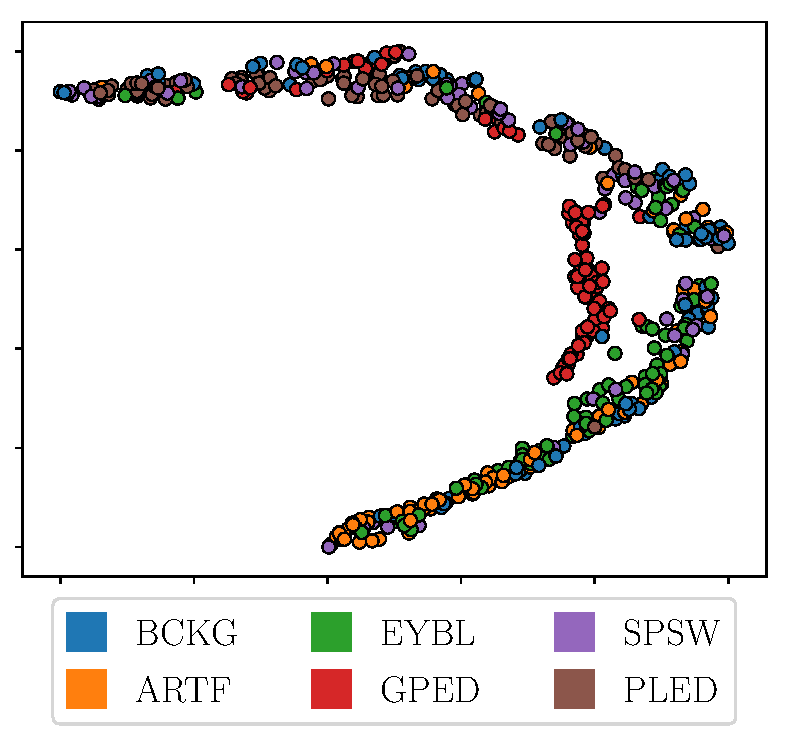
\includegraphics[width=0.55\linewidth]{pictures/tsne_plot_start.pdf}
	\caption[t-SNE visualization after $5$k iterations]{t-SNE reduced 2D visualization  of validation set for the DCNN clustering network after five thousand iterations with $\alpha = 0.5$, $\eta = 10^{-5}$ after $5$k iterations, and an accuracy of $26.6\%$ with 31-NN classification after EEG signal was passed through the DCNN clustering network}\label{fig:tsne_start}  
\end{figure}


\begin{figure}[!ht]
	\centering
	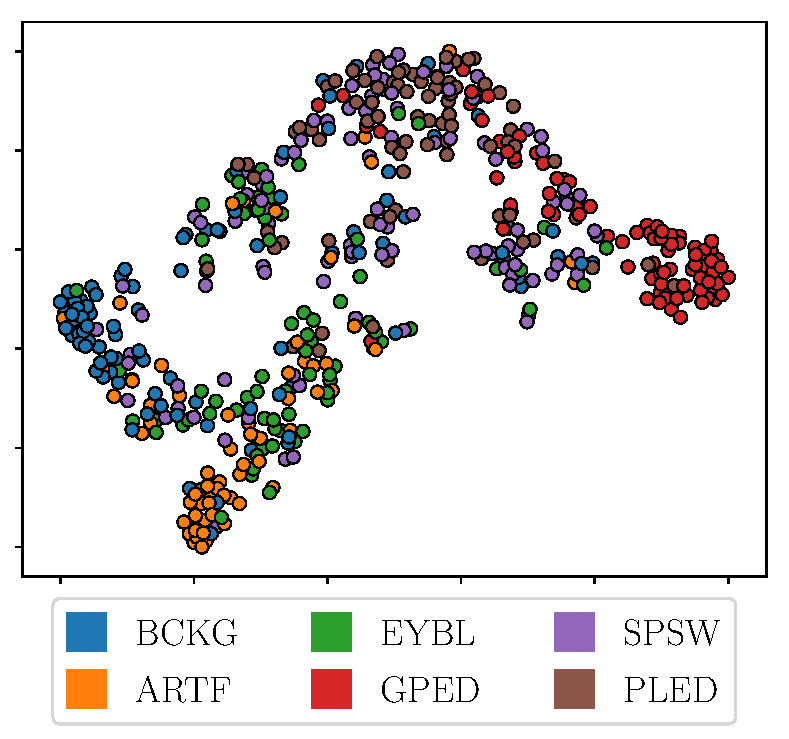
\includegraphics[width=0.55\linewidth]{pictures/tsne_plot.pdf}
	\caption[t-SNE visualization after $105$k iterations]{t-SNE reduced 2D visualization  of validation set for the DCNN clustering network with $\alpha = 0.5$, $\eta = 10^{-5}$ after $105$k iterations, and an accuracy of $60.4\%$ with 31-NN classification after EEG signal was passed through the DCNN clustering network}\label{fig:tsne}  
\end{figure}

We can see a clear difference of the t-SNE embedding after $100$k iterations. Initially, \cref{fig:tsne_start} shows that the GPED signal is separating out from the crescent in the middle but, the rest of the classes are far off from forming their own clusters and are mixed together. However, \cref{fig:tsne} shows that the clusters are forming even in a $2$-dimensional space.  GPED, BCKG and ARTF have clearly split away from each other and have formed their own clusters. 

We see a lot of qualatitative correlation between the confusion matrix in \cref{fig:dcnnlarge} and t-SNE plot in \cref{fig:tsne}. For example, according to the confusion matrix GPED was classified correctly $94\%$ of the times that it was encountered in the validation set. This makes sense since the t-SNE plot shows a large cluster of GPED signals. Hence, we can conclude that the clustering algorithm is probably working well because of the amount of qualitative correlation between the t-SNE plot and the confusion matrix.


\subsection{Comparison with a DCNN Classifier}
Another way to measure the performance of the clustering network is to compare it with a baseline algorithm. Since we are evaluating the performance of a neural network as a method of clustering EEG signals, we decided to find out how the same architecture as a classifier would perform so that we could compare their performance. In order to keep the same architecture so that we are confident that the architecture would not make a difference, we add an extra fully-connected layer to the network in \cref{tab:dcnn} as a classification layer with a softmax activation without changing anything else and trained the network on the softmax cross-entropy loss function used in neural network classifiers. We use the same exact hyperparameters as we used in training the clustering network and achieved a validation accuracy of $50.2\%$. The confusion matrix for the results of this network is shown in \cref{fig:dcnnclasslarge}. 

\begin{figure}[!ht]
	\centering
	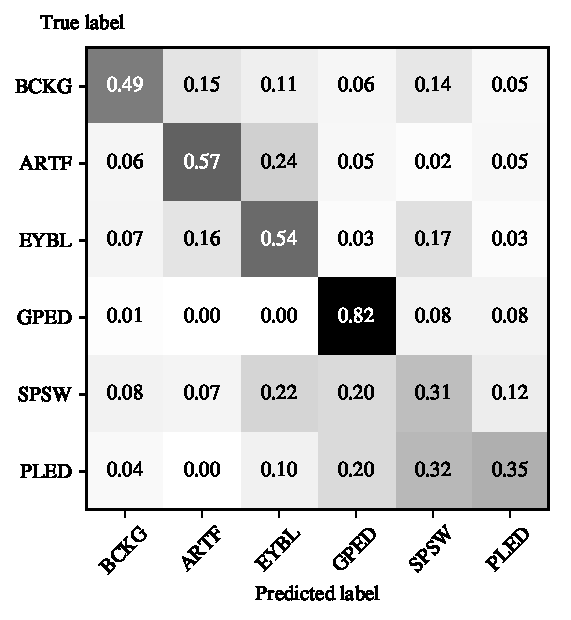
\includegraphics[width=0.55\linewidth]{pictures/conf_mat_baseline.pdf}
	\caption[Confusion matrix for the baseline DCNN classifier]{Confusion matrix for the baseline DCNN classifier with the same hyperparameters as \cref{fig:dcnnlarge} after 200k iterations and an accuracy of $50.2\%$ with $31$-NN classification}\label{fig:dcnnclasslarge}  
\end{figure}

These results were perplexing. A classifier is particularly trained on the task of discriminating between different classes whereas our clustering network is trained on the triplet loss which hoped to group similar signals together. It was surprising that a network that was trained on classification did not do better than the network that was trained on clsutering. These results suggest that it may actually better to use the triplet loss in any situation since it provides more information about the original data, can work with any number of classes and possibly detect new classes once trained, and still perform better than the DCNN on a classification task. 

Furthermore, it is likely that this phenomenon occurred directly due to the differences in loss functions since each network had nearly identical architectural forms. The features learned by the DCNN trained on the triplet loss and the features learned by the penultimate layer in the DCNN classifier are probably different because of the difference in the way the networks are trained.

\subsection{Binary Classification Using the Latent Space}

We were curious as to how well our system would work if we only used it to classify a signal as either a seizure-like signal or noise-like signal.  We considered BCKG, EYBL and ARTF as signals that are noise-like, and SPSW, GPED and PLED to be seizure-like signals as shown in \cref{tab:classes}. We can pose this as a k-NN classification problem since our network has already been trained. We found the binary classification confusion matrix as shown in \cref{fig:conf_mat_exp_pooled} and found the overall accuracy to be $90.2\%$.

\begin{figure}[!ht]
	\centering
	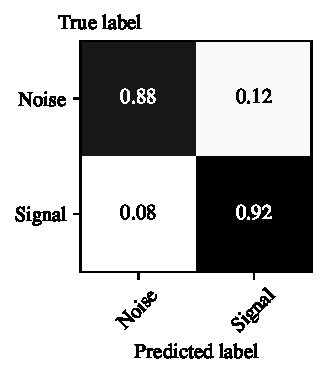
\includegraphics[width=0.425\linewidth]{pictures/conf_mat_exp_pooled.pdf}
	\caption[Binary Confusion Matrix for  the DCNN Clustering Network]{Binary confusion matrix for the DCNN clustering network with $\alpha = 0.5$, $\eta = 10^{-5}$ after $105$k iterations, and an accuracy of $90.2\%$ with 31-NN classifier}\label{fig:conf_mat_exp_pooled}
\end{figure}

\begin{figure}[!ht]
	\centering
	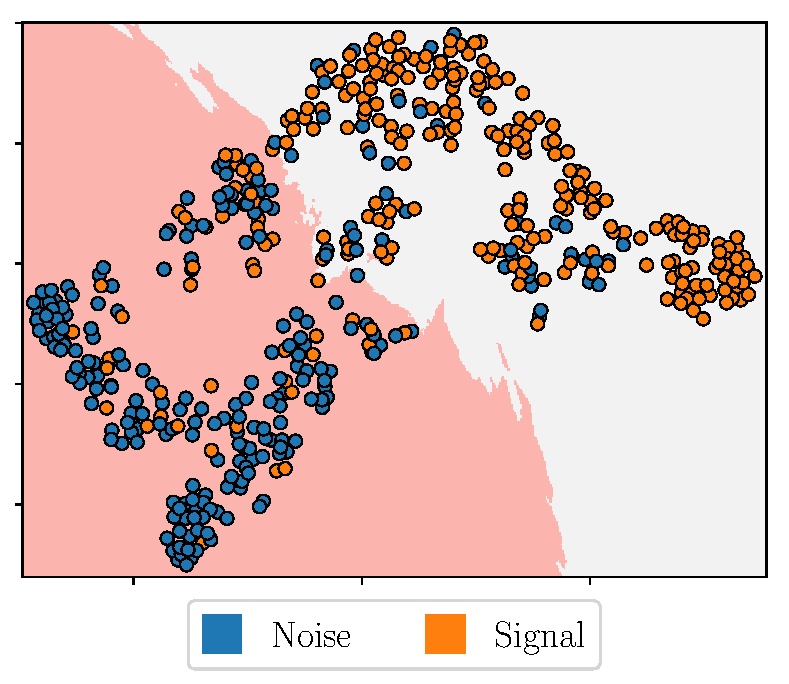
\includegraphics[width=0.55\linewidth]{pictures/tsne_plot_binary.pdf}
	\caption[k-NN Binary Decision Boundary on t-SNE Reduced Embedding]{k-NN classifier decision boundary for t-SNE reduced 2D visualization of validation set for the DCNN clustering network after five thousand iterations with $\alpha = 0.5$, $\eta = 10^{-5}$ after $105$k iterations and a 31-NN classifier}\label{fig:tsne_plot_binary}  
\end{figure}

Modifying the t-SNE to label seizure-like signals and noise-like signals, and plotting the decision boundary of a k-NN classifier as shown in \cref{fig:tsne_plot_binary} demonstrates that there is a boundary that separates seizure-like signal from noise-like signal clearly. Even though we trained on all types of triplets (e.g. PLED-PLED-GPED, GPED-GPED-BCKG etc.), we still found a clean separation between seizure-like signals and noise-like signals. This phenomena demonstrates that not only are the set of triplet classes that we train on separating, but their super classes, i.e. the general signal types, are separating which can possibly lead to a better, hierarchical taxonomy. 

%\subsection*{Using Different Metrics}


\section{Analysis on Seizure-Like \& Noise-Like Files}
\label{analysis}
Although our network has done quite well on a rather noisy dataset, a thorough error analysis is certainly the most important step in order to determine how to pivot. In order to do so, we analyzed how the network does on subsets of the data and tried to discover any patterns or explanations that might help us improve the network in order to get better results. We split the data into the following three subsets: 
\begin{itemize}
	\setlength\itemsep{1mm}
	\item sessions without sessions without seizure-like signals
	\item sessions with seizure-like signals
  	\item sessions with seizure-like signals considering only seizure-like signals
\end{itemize}
   
We were able to separate the different signals based on their original session and what types of signals existed in that session. Everytime we computed a confusion matrix for validating the network on the stratified sampled dataset, we also computed a confusion matrix for a stratified sampled subset of the dataset for each of the above categories. In doing so, we obtained the following results. 

\begin{figure}[!ht]
	\centering
	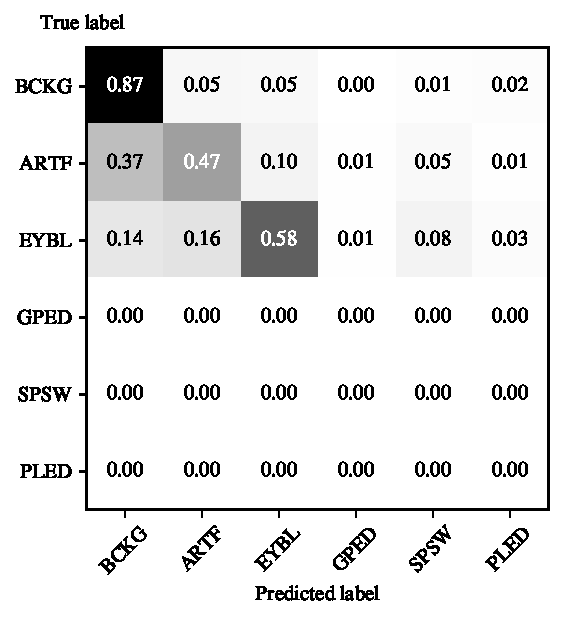
\includegraphics[width=0.55\linewidth]{pictures/conf_mat_exp_without_seizure.pdf}
	\caption[Confusion Matrix on Sessions without Seizure-Like Signals]{Confusion matrix of DCNN clustering network on files without seizures resulting in an accuracy of $64.6\%$ with $\alpha = 0.5$, $\eta = 10^{-5}$ after $105$k iterations and a 31-NN classifier}\label{fig:conf_mat_exp_without_seizure}  
\end{figure}

The confusion matrix shown in \cref{fig:conf_mat_exp_without_seizure} is on the data from sessions that do not contain any seizure-like signals. These sessions only contain BCKG, ARTF and EYBL signals. Hence, the bottom half of the confusion matrix is empty. The right half of the confusion matrix is not completely empty because the DCNN along with the k-NN classifier still predicts some of these signals to be GPED, SPSW or PLED since the network is still trained on the training set which contains all the classes. These incorrect predictions are expected to occur due to various sources of natural background noise, and incorrect true labels or shared characteristics that are closer to seizure-like signals as opposed to noise-like signals. This results in a $64.6\%$ overall accuracy after $105$k iterations.

\begin{figure}[!ht]
	\centering
	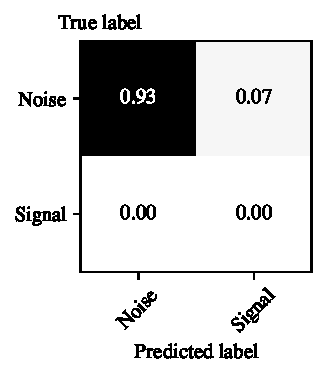
\includegraphics[width=0.425\linewidth]{pictures/conf_mat_exp_without_seizure_pooled.pdf}
	\caption[Binary Confusion Matrix on Sessions without Seizure-Like Signals]{Binary classification confusion matrix of DCNN clustering network on files without seizures resulting in a binary accuracy of $93.0\%$ with $\alpha = 0.5$, $\eta = 10^{-5}$ after $105$k iterations and a 31-NN classifier}\label{fig:conf_mat_exp_without_seizure_pooled}  
\end{figure}

As we had done before, we had also made a binary confusion matrix as well. Just like the confusion matrix presented in \cref{fig:conf_mat_exp_without_seizure}, the bottom half of the confusion matrix is empty and the top-right of the confusion matrix is not empty. The system achieved a $93\%$ accuracy in detecting that a second of signal is noise-like and not a seizure-like signal. In other words, given only noise-like signals, we are able to classify 93\% of those signals as noise-like signals using our system and the 7\% as not noise-like (i.e. seizure-like) signals. 

The confusion matrix in \cref{fig:conf_mat_exp_with_seizure} is on sessions that contain seizure-like signals. Sessions that contain seizure-like signals also contain noise-like signals since the entire session is not full of seizure-like signals. Therefore, all the types of signals are present in the confusion matrix. However, these sessions are mutually exclusive from the sessions that we looked at in \cref{fig:conf_mat_exp_without_seizure} since those sessions do not contain any seizure-like signals at all. When looking at sessions that contain seizure-like signals, we obtained an overall accuracy of $56\%$ after $105$k iterations.

\begin{figure}[!ht]
	\centering
	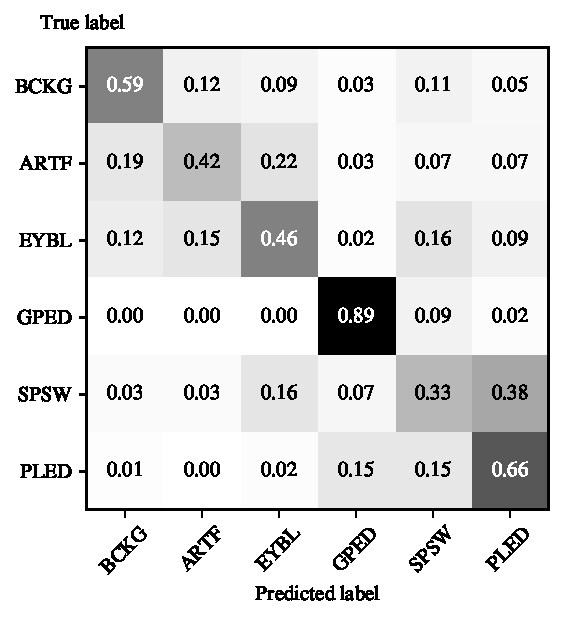
\includegraphics[width=0.55\linewidth]{pictures/conf_mat_exp_with_seizure.pdf}
	\caption[Confusion Matrix on Sessions with Seizure-Like Signals]{Confusion matrix of DCNN clustering network on files with seizures resulting in an accuracy of $56.0\%$ with $\alpha = 0.5$, $\eta = 10^{-5}$ after $105$k iterations and a 31-NN classifier}\label{fig:conf_mat_exp_with_seizure}  
\end{figure}

Like before, we also constructed a binary classification confusion matrix. In this case, given that the session contains a seizure, we are able to classify the signal as seizure-like or noise-like with an accuracy of 85\%. The noise-like signals were able to be detected correctly with a 78\% accuracy and the seizure-like signals were able to be detected correctly with a 91\% accuracy. 


\begin{figure}[!ht]
	\centering
	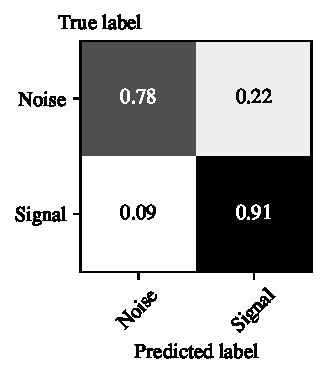
\includegraphics[width=0.425\linewidth]{pictures/conf_mat_exp_with_seizure_pooled.pdf}
	\caption[Binary Confusion Matrix on Sessions with Seizure-Like Signals]{Confusion matrix of DCNN clustering network on files with seizures resulting in an accuracy of $85.0\%$ with $\alpha = 0.5$, $\eta = 10^{-5}$ after $105$k iterations and a 31-NN classifier}\label{fig:conf_mat_exp_with_seizure_pooled}  
\end{figure}

Finally, the confusion matrix in \cref{fig:conf_mat_exp_with_only_seizure} is on sessions that contain seizure-like signals but excluding noise-like signals to explore how the system performs on just signals that have seizures (i.e. GPED, SPSW, PLED). This is why the top half of the confusion matrix is empty and we see that most of the predictions are within the bottom right square of the confusion matrix, which is what we expected. Note that the signals that were tested to produce this confusion matrix are not necessarily mutually exclusive from the signals that we tested in \cref{fig:conf_mat_exp_with_seizure} since the signals used to form that confusion matrix were the ones that contained seizures. The experiment results in an overall validation accuracy of $60.4\%$ after $105$k iterations. We also see that a lot of the SPSW are being classified as PLED. This is likely because of the high similarity between PLED and SPSW.

\begin{figure}[!ht]
	\centering
	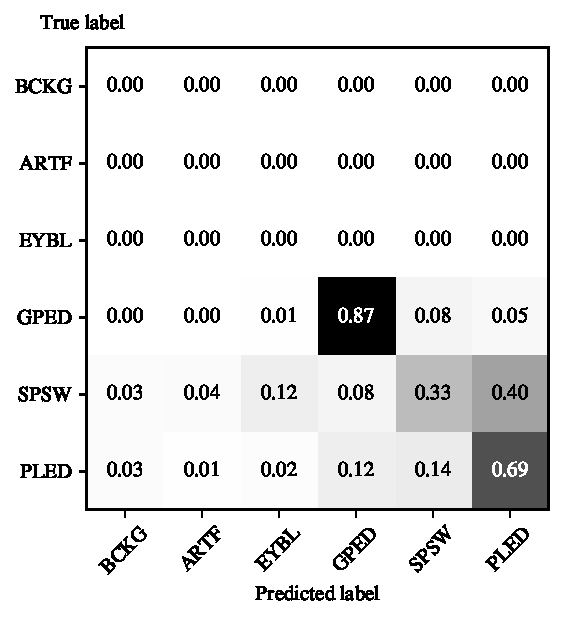
\includegraphics[width=0.55\linewidth]{pictures/conf_mat_exp_with_only_seizure.pdf}
	\caption[Confusion Matrix on Sessions with only Seizure-Like Signals]{Confusion matrix of DCNN clustering network on files with ONLY seizure signals resulting in an accuracy of $63.0\%$ with $\alpha = 0.5$, $\eta = 10^{-5}$ after $105$k iterations and a 31-NN classifier}\label{fig:conf_mat_exp_with_only_seizure}  
\end{figure}

\begin{figure}[!ht]
	\centering
	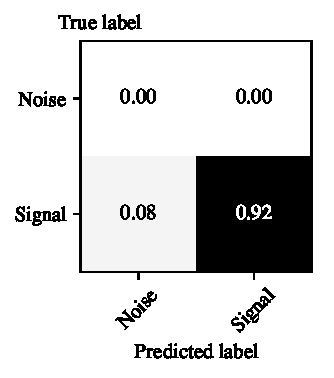
\includegraphics[width=0.425\linewidth]{pictures/conf_mat_exp_with_only_seizure_pooled.pdf}
	\caption[Binary Confusion Matrix on Sessions with only Seizure-Like Signals]{Confusion matrix of DCNN clustering network on files with ONLY seizure signals resulting in an accuracy of $91.8\%$ with $\alpha = 0.5$, $\eta = 10^{-5}$ after $105$k iterations and a 31-NN classifier}\label{fig:conf_mat_exp_with_only_seizure_pooled}  
\end{figure}

Similar to the last experiment, we also generated a binary classification confusion matrix. Given that the session contains a seizure and we are only looking at seizure signals in that particular session, we are able to observe that the signal presented to the system is seizure-like 92\% of the time and mis-classified the signal as noise 8\% of the time. 

In doing the analysis on the subsets of the validation set, it is revealed that most of the error in attempting to recognize a signal as a one of the types of seizure-like signals arises because the signal is classified as one of the other types of seizure-like signals. For example, if a signal with PLED as the true label is presented to the system and the system makes an error in predicting the label of the signal, it is likely for the prediction to be SPSW or GPED as opposed to the noise-like signals. A possible reason for this phenomena may be because the given signal is more similar to SPSW or GPED. This phenomena is alright because the system is expected to cluster and place similar signals near each other. Logically this makes sense since the seizure-like signals are expected to be more similar to each other than noise-like signals. The binary confusion matrices supports this since it has a high true positive rate and a true negative rate. 

Another common error that was seen in the various confusion matrices was the relatively high false classification rate of SPSW signals as PLED. This error could be attributed to the similarity between SPSW and PLED, however, it is also likely that amount of data present on SPSW is not enough. Furthermore, we may have also made an error when filtering the raw signal with a pass-band of $1$ Hz to $70$ Hz. SPSW by definition has high frequencies. It may be possible that some of these high frequencies are above $70$ Hz. The assumption that the bulk of the signal is between that pass-band may be false in this case. 


% \section{Using Recurrent Networks}

% Although most of our work was in using convolutional neural networks to build a latent space, we briefly explored whether we could use recurrent neural networks (RNNs \nomenclature{RNN}{Recurrent Neural Networks}) to do the same. RNNs are a class of computational graphs that feedback the current after 105k iteration output of a neuron back to its predecessors or itself such that the future outputs are dependent on the current output as well as the past outputs. Recurrent neural nets have been shown to perform well on sequential data and time-dependent data as demonstrated by \citet{}. 

% Given that the spectrogram that we derived from the TUH EEG corpus still maintains time dependent information as seen in \cref{fig:stft}, it might be helpful to use a recurrent neural network as opposed to a convolutional neural network for the same task. In particular, the Long Short-Term Memory (LSTM \nomenclature{LSTM}{Long Short-Term Memory}) units instead of the generic RNN since they were made to retain information for a longer time and avoid the vanishing gradient problem. 	11
